\documentclass[main.tex]{subfiles} % Subfile-Class

%==============================================================================%
%                                   Subfile                                    %
%==============================================================================%

\begin{document}

\subsection{Informatik}

\paragraph{Einleitung}

Das Informatik-Teilsystem bildet das "Gehirn" unseres Fahrzeugs:
Es verknüpft Sensorik, Aktorik und die übergeordneten
Wettbewerbslogiken und stellt sicher, dass alle Funktionsblöcke
deterministisch zusammenarbeiten.
Kernstück ist ein \emph{Raspberry Pi Hat} auf welchem die
Linux-Distribution Ubuntu läuft, das über ein
eigenes 64bit UART-Protokoll mit dem \emph{Motion-Controller}
und dem \emph{Grip-Controller} kommuniziert.
Die steuernde Software ist ein in Python implemeniertes Program, welches modular
aufgebaut ist und die verschiedenstens Subprogramme wie auch das
Hauptprogramm enthält.

Die folgenden Unterkapitel geben einen detaillierten Überblick über
die zentralen Softwarekomponenten:

\begin{itemize}\setlength\itemsep{0.3em}
  \item \textbf{Änderungen zu PREN1} - architektonische Anpassungen
    und Refactorings, die sich durch neue bzw. bessere Erkentnisse
    herauskristallisiert haben.
  \item \textbf{Bilderkennung mit Kamera} - beschreibt die Implementierung
    der Bildverarbeitung mittels OpenCV auf der \emph{Raspberry Pi
    Camera} und den Algorithmen zur Objekterkennung.
  \item \textbf{UART-Protokoll} - ein festes 64bit Frame mit
    8-Bit-CRC zur robusten, latenzarmen Punkt-zu-Punkt-Kommunikation
    zwischen den Teilsystemen.
  \item \textbf{Wegfinde-Algorithmus} - Beschreibung unserer
    Zustandsmaschine, die den Pfadfindungsalgorithmus implementiert,
    der das Fahrzeug autonom zu einem der drei Ziele navigiert.
\end{itemize}

Gemeinsam bilden diese Bausteine eine robuste, erweiterbare
Plattform, die alle funktionalen (Wegplanung, Objektmanipulation
mittels Greifers) und
nicht-funktionalen (Fehlertoleranz, Wartbarkeit)
Anforderungen des Projekts erfüllt.

Folgendes Komponentenmodell visualisiert die Beziehungen
zwischen unseren einzelnen Softwarekomponenten:

\begin{figure}[H]
    \centering
    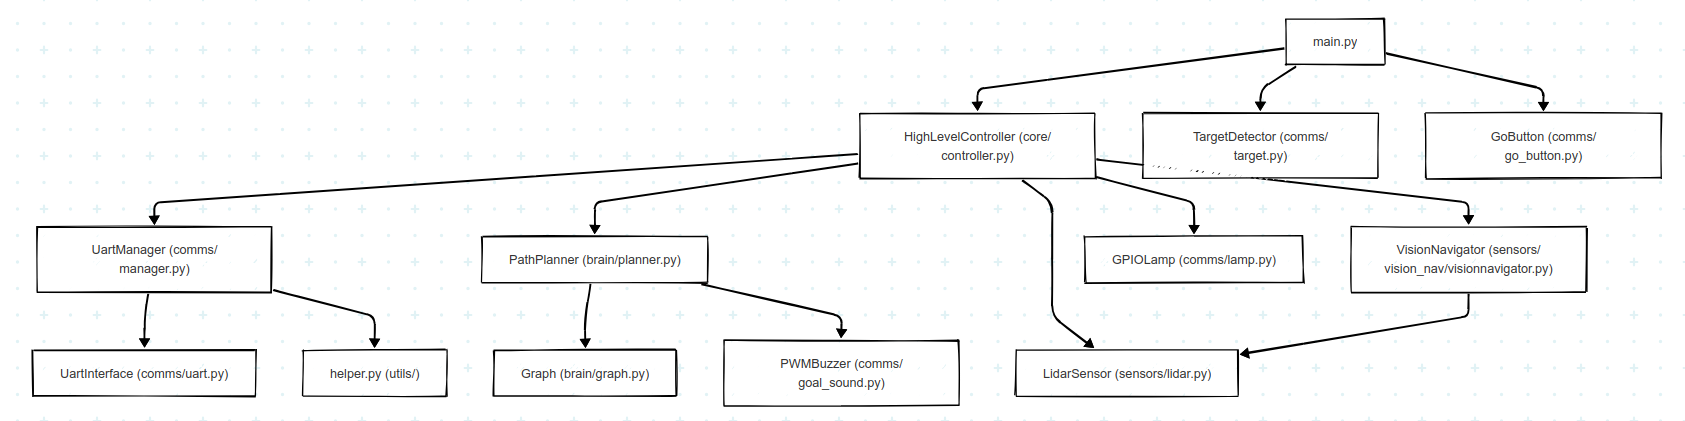
\includegraphics[width = 0.9\linewidth]{./Informatik_subfiles/fig_Informatik/diagram_not_fucked.png}
    \caption{Komponentenmodell der Software auf dem RaspberryHAT}~\label{fig:Komponentenmodell}
\end{figure}

\subfile{./Informatik_subfiles/Wegfinde_Algorhytmus.tex}
\newpage

\subfile{./Informatik_subfiles/Uart_Protokoll.tex}
\newpage

\subfile{./Informatik_subfiles/Bilderkennung_mit_Kamera.tex}
\newpage

\subfile{./Informatik_subfiles/Aenderungen_zu_konzept_PREN1.tex}
\newpage

\end{document}
